\section{Linguistic Analysis}

Sawicki et al. 2023's survey \cite{sawicki_state_2023} tell us that English is by far the most represented language in the field of natural language processing. Fortunately, French and Italian are still in the top eight (figure \ref{fig:lanpop}), so finding libraries already capable of handling them should be easy enough. It is worth noting that results could be biased since the authors looked for papers written in english.

\begin{figure}[h]
  \centering
  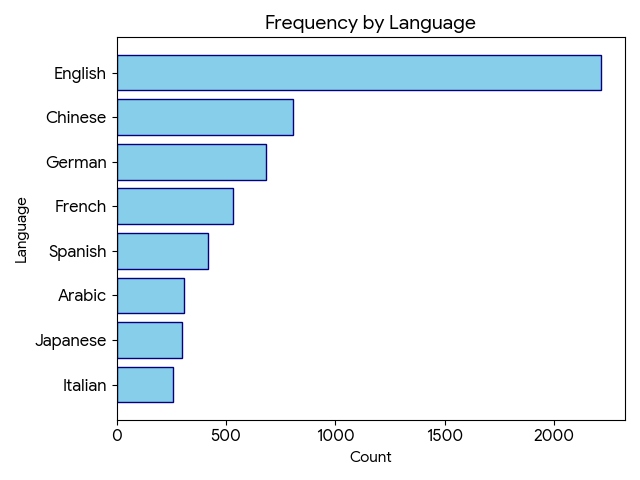
\includegraphics[width=.7\linewidth]{images/sawicki_languagesPopularity.png}
  \caption{Most popular language in the field of Natural Language Processing \cite{sawicki_state_2023}}
  \Description{English is at 2000 count popularity, Chinese second most popular at 700. Italian least popular at 300.}
  \label{fig:lanpop}
\end{figure}

The pipeline for pre-processing is quite standard, and it involves, among other steps, removing stop words, Part-Of-Speech tagging, tokenization and lemmatization, as well as building the text embeddings. 

\textbf{FastText}\footnote{FastText is a lightweight library for efficient text classification and representation learning: \url{https://fasttext.cc/}.} is an open-source, free, lightweight library that allows users to learn text representations and text classifiers that gained a lot of popularity especially for its performances in computing text embeddings. 

\textbf{LLM2Vec} \cite{behnamghader_llm2vec_2024} is a recipe to convert decoder-only LLMs into text encoders, so that they can be used to generate state-of-the-art text embeddings.

\textbf{Stanza}\footnote{Stanza – A Python NLP Package for Many Human Languages: \url{https://stanfordnlp.github.io/stanza/index.html}.} is a collection of accurate and efficient tools for the linguistic analysis of many human languages. Starting from raw text, Stanza divides it into sentences and words, and then can recognize parts of speech and entities, do syntactic analysis, and more. Stanza brings state-of-the-art NLP models to languages of your choosing.

\textbf{spaCy}\footnote{spaCy, an Industrial-Strength Natural Language Processing: \url{https://spacy.io/}.} is another well known and powerful NLP library for Python that supports multiple languages. Moreover, it supports tokenization, part-of-speech tagging, dependency parsing, sentence segmentation, text classification and lemmatization. It supports multi-task learning with pretrained transformers and has pretrained word vectors. It supports custom models in PyTorch and Tensorflow, and has built in syntax visualizers.

\textbf{simplelemma}\footnote{simplelemma is a lightweight toolkit for multilingual lemmatization and language detection: \url{https://pypi.org/project/simplemma/}.} is also worth mentioning as a lightweight Python lemmatizer.

\textbf{textacy}\footnote{textacy: NLP, before and after spaCy. \url{https://pypi.org/project/textacy/}.} is a Python library for performing a variety of natural language processing (NLP) tasks, built on spaCy and intended to be used before it (pre-processing step) and after it (NLP step). Assesses text complexity with Flesch-Kincaid readability test and text diversity with Type-Token Ratio. 

Text complexity can also be measured with \textbf{TRUNAJOD}\footnote{TRUNAJOD: A text complexity library for text analysis built on spaCy. \url{https://trunajod20.readthedocs.io/en/latest/}.}, another spaCy-based Python library that implements synonym overlap, coherence between sentences and other metrics. 

On the matter of populism and hate speech classification, there are a lot of transformer-based models from \textbf{Hugging Face}\footnote{Hugging Face, Inc., is an American company based in New York City that develops computation tools for building applications using machine learning. Its transformers library built for natural language processing applications and its platform allow users to share machine learning models and datasets and showcase their work. \url{https://huggingface.co/}}. Some examples follow.

\begin{itemize}
    \item English: \url{https://huggingface.co/Hate-speech-CNERG/dehatebert-mono-english};
    \item French: \url{https://huggingface.co/Hate-speech-CNERG/dehatebert-mono-french};
    \item Italian: \url{https://huggingface.co/Hate-speech-CNERG/dehatebert-mono-italian}.
\end{itemize}

There are transformer based on roBERTa for both hate speech and populism classification, for example here follows a 0.4 billion parameters model based on Trump speeches: \url{https://huggingface.co/coastalcph/roberta-large-ft-trump-populism}.

Hate speech can also be detected with the Python library \textbf{HateSonar}\footnote{HateSonar: Hate Speech Detection. \url{https://pypi.org/project/hatesonar/}.} which uses a BERT based model.

\subsection{Speech To Text}

\TODO
%% tutto sbagliato ho trovato libreri text to speech e non speech to tex

Since there are plenty of video and audio speeches publicly available, they could be integrated in the corpus after translating them into text. This can be easily achieved with either \textbf{gTTS}\footnote{gTTS (Google Text-to-Speech), a Python library and CLI tool to interface with Google Translate text-to-speech API. \url{https://pypi.org/project/gTTS/}.} or \textbf{SpeechT5}\footnote{SpeechT5 model fine-tuned for speech synthesis (text-to-speech) on LibriTTS. \url{https://huggingface.co/microsoft/speecht5_tts}.} libraries: the former is a Google-based text-to-speech Python library with a command line interface, the latter is a Hugging Face library based on Microsoft S-t-T pre-trained model. Both can be installed via \texttt{pip}.